\chapter{低精度分布式更新算法}
本章主要介绍低精度分布式更新(LPDU)算法的实现原理,并详细介绍整个框架工作流程和性能优化的相关方法。通过分析不同应用的理论效率和实际效率结果,评估系统的性能。
\section{引言}
随着人工智能的快速发展,为提升训练效率,满足生产需求,业界已针对分布式深度学习系统进行了深入的研究。本章提出的LPDU算法希望通过低精度数据通信方法来减少分布式同步数据过程中的数据传输量,从而减小同步时间开销,提高分布式训练效率;同时,为保证神经网络的训练精度,使用混合精度更新方法对网络进行更新。本章将介绍如何在现有高效的分布式通信框架horovod上集成现有主流的深度学习框架,并进一步实现LPDU算法,分析低精度数据通信相对于原始浮点数通信的缺点,以及对应的改进方法;并介绍相关的优化方法,最后通过理论分析和实验结果比较,说明LPDU算法的有效性和实用性。
\section{MXNet与Horovod的整合}
horovod是uber针对tensorflow在分布式深度学习训练中的不足,基于百度提出的ring-allreduce构建。有3个主要特征:

1. horovod与深度学习框架相互独立,用户以python包的形式调用horovod的API。使其发展独立于任何深度学习框架,目前horovod已经支持tensorflow和pytorch。这样tensorflow和pytorch用户可以在任意版本的深度学习框架中使用horovod,不需要担心兼容问题。目前MXNet团队已经将MXNet整合进了horovod,正在等待horovod团队整合。

2. 用NCCL取代百度ring-allreduce实现。NCCL是NVIDIA的通信库,提供高度优化的ring-allreduce实现。通过NCCL的ring-allreduce实现,使得horovod的性能有巨大提升。

3. 提出tensor fusion方法,通过将多个小的tensor整合成数据量稍大的tensor,进而对这个大的tensor做allreduce。提高了数据的通信效率。

\begin{figure}[htp]
\centering
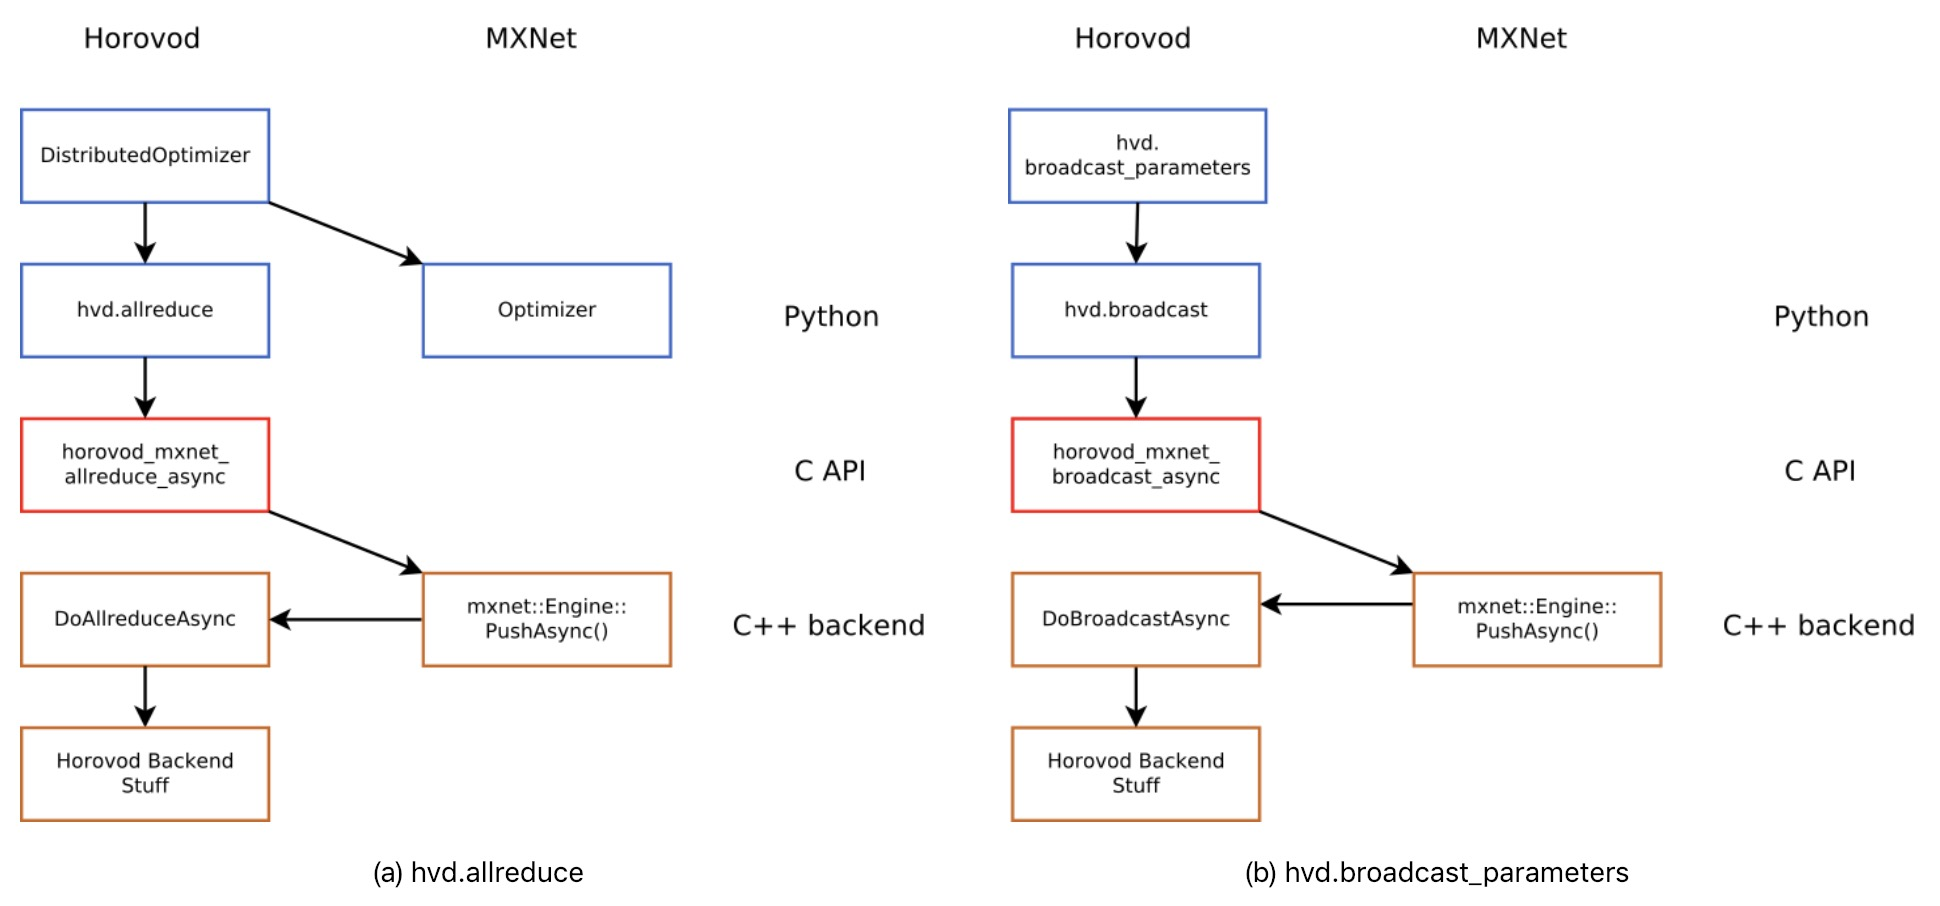
\includegraphics[width=12cm]{horovod_mxnet_integration}
\caption{MXNet与horovod整合示意图}
\label{fig:horovod_mxnet_integration}
\end{figure}
horovod中主要涉及两个操作:allreduce和broadcast。其与MXNet的整合示意图如图~\ref{fig:horovod_mxnet_integration}所示。由图可知,horovod通过继承MXNet的优化器optimizer实现与MXNet的整合,即更新模型时使用horovod的DistributedOptimizer更新。对于MXNet而言,分布式程序只是一个使用DistributedOptimizer优化器更新模型的单机程序。在horovod中,因为其在真正更新之前,会对参数做allreduce来同步全局参数。这种整合方式使得MXNet与horovod可以各自独立发展,而不会产生版本的相互依赖。为保证各个节点中初始化的模型一致, 其提供了一个broadcast parameters的API用于同步模型初始化的值。

horovod通过对外提供tensor接口,各个深度学习框架通过继承该tensor接口,提供自身的实现即可整合到horovod中。接口如下所示:

\begin{lstlisting}[language=C, numbers=none]
Tensor {
  dtype();  //  return the data type of tensor;
  shape();  //  return the shape of tensor;
  data();   //  return the data pointer of tensor;
  size();   //  return the total bytes of data;
}
\end{lstlisting}

由上伪代码可知,将深度学习框架整合进horovod只需通过继承tensor这个基类并实现对应的方法即可。而horovod只需通过调用tensor中的对应方法即可完成数据的同步。故为将MXNet整合入horovod,其设计如下:

\begin{lstlisting}[language=C, numbers=none]
MXTensor : Tensor{
public:
  MXTensor(NDArray* tensor);
  // override the 4 APIs
  dtype();
  shape();
  data();
  size();
protected:
  NDArray* tensor_;  // the pointer address to the data from MXNet
}
\end{lstlisting}

\section{LPDU算法的设计与实现}
\begin{figure}[htp]
\centering
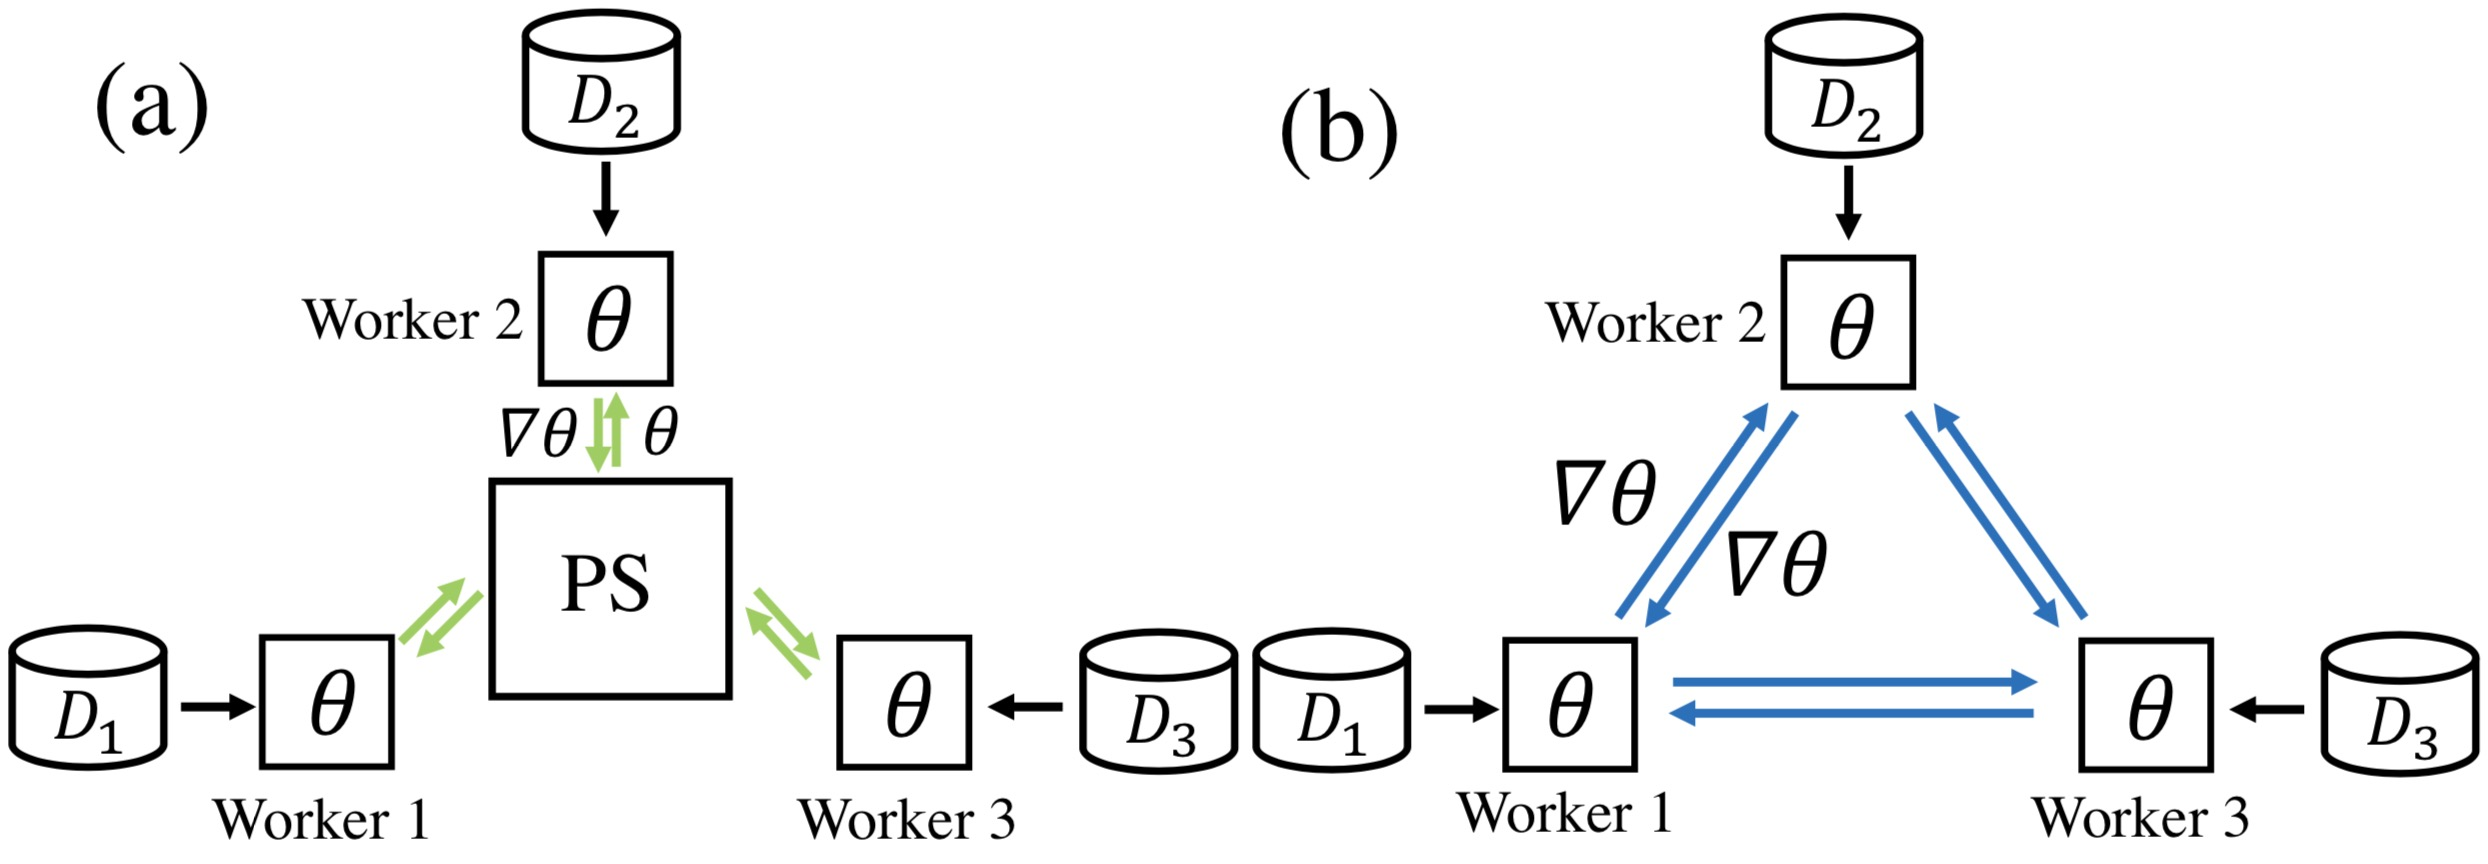
\includegraphics[width=13cm]{ps_allreduce}
\caption{PS(a)和MPI(b)下数据并行的实现原理}
\label{fig:ps_allreduce}
\end{figure}

在数学形式上,给定数据集$D$,损失函数$L$,拟合参数为$\theta$的神经网络的过程,可以被建模成公式~\ref{equ:nn_equ}形式。其中$t$表示迭代次数,$\nabla L$表示在当前参数$\theta^{(t-1)}$,数据为$D^{(t)}\subset D$,学习率为$\epsilon$时,损失函数的梯度。在不断迭代过程中,直至$\theta$达到终止要求。
\begin{equation}
\label{equ:nn_equ}
\theta^{(t)}=\theta^{(t-1)}+\varepsilon\cdot\nabla L(\theta^{(t-1)},D^{(t)})
\end{equation}

在分布式深度学习中,通常采用数据并行的方式进行分布式训练,其通过将数据集$D$划分,放在不同计算节点(下标为$p=1,...,P$)上,如图~\ref{fig:ps_allreduce}所示。在每次迭代$t$中,每个计算节点从各自数据集$D_{p}$获取单次迭代数据$D^{(t)}_{p}$,并计算模型梯度$\nabla L(\theta^{(t)},D^{(t)}_{p})$;随后系统将各个节点梯度进行聚合,使用下列公式~\ref{equ:nn_dl_equ}对模型进行更新。
\begin{equation}
\label{equ:nn_dl_equ}
\theta^{(t+1)}=\theta^{(t)}+\varepsilon\sum^{P}_{p=1}\nabla L(\theta^{(t)},D^{(t)}_{p})
\end{equation}

在数据并行模式下,每个计算节点都要在本地维护一份全局共享参数$\theta$,这将产生大量的通信开销。目前主要有参数服务器(图~\ref{fig:ps_allreduce}a)和MPI(图~\ref{fig:ps_allreduce}b)两种方法来实现全局参数的维护。本章算法则是基于MPI通信模式提出。假设神经网络模型参数$\theta$的数据量为$M$,由图~\ref{fig:ps_allreduce}b可知,在每次迭代$t$中,每个worker会发送、接受模型当前梯度$\nabla\theta$,其大小与模型参数$\theta$相同,即每个worker都会产生$2M$的通信数据量。该通信数据量大小对分布式训练神经网络的效率影响至关重要。本章LPDU算法针对神经网络自身的容错性及其对数据精度不敏感的特点,将32比特浮点数表示的梯度数据$\nabla\theta$转换成16比特的bfloat16数据格式,使得$\nabla\theta$的数据量由$M$减少至$M/2$。此时,每次迭代$t$中每个worker传输的数据量从$2M$减少至$M$,使得分布式系统的通信开销降低,提升系统训练效率。且神经网络参数$\theta$的数据量越大,提升效果越明显。

LPDU算法主要包含两部分:低精度数据通信和混合精度更新。低精度数据通信部分旨在减少分布式训练过程中的同步通信开销,从而提升分布式训练效率;混合精度更新部分则是为避免低精度数据表示带来的数据精度损失造成神经网络训练精度下降的问题,将同步后的低精度梯度数据转换为原始浮点数,再对网络进行更新,可减小更新过程中的数据损失。使用该方法可保证在低精度数据通信情况下神经网络训练精度达到原始浮点数训练的相同精度。
\subsection{低精度数据通信算法}
%分析在训练过程中梯度的分布范围。确定在该范围内,浮点数与bf16数据的精度差距。

由2.1部分可知,相对于单机训练,分布式训练多了额外的同步通信开销,其对分布式训练效率的高低有至关重要的作用。结合业界对低精度数据在神经网络中的研究进展,本节提出一种高效的低精度数据通信方法,在混合精度更新算法配合下,能在不损失神经网络训练精度的情况下,提升分布式训练效率。

算法核心思路是:使用低精度数据进行通信,相对于浮点数通信减少了一半数据量,从而提升训练效率。根据业界对低精度数据在神经网络中的研究进展可知,目前主要有两种低精度数据格式用于神经网络训练,分别是半精度浮点数(FP16)和bfloat16(BF16)数据格式。两种在表示数值范围和精度上均有不同程度的损失,通过对应的改进方法,可保证低精度数据下神经网络的训练精度达到原始浮点数训练相同精度。

考虑到FP16与BF16数据格式的特点,BF16数据格式与浮点数之间的转换开销较小,且其可表示的数值范围与浮点数基本相同,故不需要考虑FP16表示情况下梯度数据超过数值表示范围的问题。基于以上两种原因,LPDU算法采用BF16格式数据进行通信,算法内容如算法~\ref{alg:lpdc_alg}所示。下面介绍基于BF16格式的低精度数据通信算法的具体实现。

\begin{algorithm}\small
\caption{低精度数据通信算法LPDC}
\textbf{输入:}
浮点数数据:$Data_{fp32}$ \\
\textbf{输出:} 
全局同步后的低精度数据:$Data_{bf16}$
\begin{algorithmic}[1]
	\STATE{将原始32比特的浮点数$Data_{fp32}$转换为BF16格式的低精度数据$Data_{bf16}$}
    \STATE{使用$allreduce$对$Data_{bf16}$做全局同步}
    \STATE{返回全局同步后的低精度数据$Data_{bf16}$}
\end{algorithmic}
	\label{alg:lpdc_alg}
\end{algorithm}

基于BF16格式的低精度数据通信算法的实现主要包含两部分:1.在进行同步之前将原始浮点数转换成BF16格式数据;2.对BF16格式的梯度数据进行同步,求得全局梯度。本文在horovod基础上对低精度数据通信算法进行实现,具体工作包括:1.继承horovod提供的Tensor类,设计BF16 Tensor,供horovod调用,其需要完成原始浮点数到BF16格式数据的转换工作;2.扩展MPI,使其支持BF16格式数据同步,实现一个自定义的BF16求和函数,供MPI在做allreduce过程中对BF16数据求和使用。

针对以上两部分内容,具体设计如下所示。在MXTensor基础上,添加了新的BF16指针,用于存放BF16数据。在构造函数中,将深度学习框架传入的FP32的数据转换成BF16数据。针对第二点BF16的求和函数的实现。因为目前没有BF16的硬件计算单元,求和计算只能在浮点计算单元上计算。由下BF16 sum函数可知,函数主要分为三部分:1.将BF16数据转换为浮点数;2.对浮点数据进行求和;3.将求和后的浮点数结果转换为BF16数据。

\begin{lstlisting}[language=C, numbers=none]
// 1. bf16 tensor defination
MXBF16Tensor: MXTensor {
public:
  MXBF16Tensor(NDArray* tensor):MXTensor(tensor){
  // according the count of tensor elements allocate memory to store bf16 data;
  // convert source data of tensor to bf16 data format
}
  source_data();   // return the source pointer of NDArray;
  // override the 3 APIs as below:
  dtype();  // return bf16 flag;
  data();    // return data pointer of bf16;
  size();     // return the total bytes of bf16 data;
  private:
  unsigned short* bf16dptr_;
}

// 2. implement bf16 sum according MPI_op define
void bf16_sum(void* invec, void* inoutvec, int* len, MPI_Datatype* datatype) {
  for(int i = 0; i < *len; i++) {
    float tmp_in = convert_bf16_to_fp32(invec[i]);
    float tmp_out = convert_bf16_to_fp32(inoutvec[i]);
    tmp_out += tmp_in;
    inoutvec[i] = convert_fp32_to_bf16(tmp_out);
  }
}
\end{lstlisting}


\subsection{混合精度更新算法}
由表1.2可知,BF16格式数据有效数字仅有2~3位,相对于FP32格式数据存在一定精度损失。由随机梯度下降(SGD)更新算法公式~\ref{equ:sgd}可知,SGD将当前梯度乘以学习率$\eta$,再将值更新到模型参数$W$中。通常情况下$\eta$是一个小于1的数,并随着训练的进行,学习率$\eta$逐渐减少。若将$\eta*g_{t,i}$存放在BF16数据格式中,该过程将造成一定的精度损失,产生计算误差,最终该误差将传播到模型参数中。
\begin{equation}
\label{equ:sgd}
W_{t+1,i}=W_{t,i}-\eta*g_{t,i}
\end{equation}

为避免更新过程中产生的精度损失,本文借鉴FP16训练神经网络的方法,使用混合精度更新算法来对模型进行更新。如算法~\ref{alg:mpu_alg}所示。其核心思想是:在更新之前将BF16格式梯度数据转换成浮点数据格式,再使用浮点数梯度对网络模型进行更新,从而避免更新过程中产生的精度损失。混合精度更新算法下,神经网络训练流程如图~\ref{fig:MPUflow}所示。可知混合精度更新算法主要分为两部分:全局同步后的BF16格式梯度到浮点数的转换和SGD算法更新。

\begin{algorithm}\small
\caption{混合精度更新算法MPU}
\textbf{输入:}
本地网络层浮点参数:$Weight_{fp32}$,全局同步后的低精度梯度:$gradient_{bf16}$ \\
\textbf{输出:} 
更新后的网络层浮点参数:$Weight_{fp32}$
\begin{algorithmic}[1]
    \STATE{将全局同步后的低精度梯度$gradient_{bf16}$转换为32比特的浮点数梯度$gradient_{fp32}$}
    \STATE{使用更新算法(如随机梯度下降算法),把转换后的浮点梯度$gradient_{fp32}$更新到网络层参数$Weight_{fp32}$中}
    \STATE{返回更新后的参数$Weight_{fp32}$用于下一次迭代训练}
\end{algorithmic}
	\label{alg:mpu_alg}
\end{algorithm}

\begin{figure}[htp]
\centering
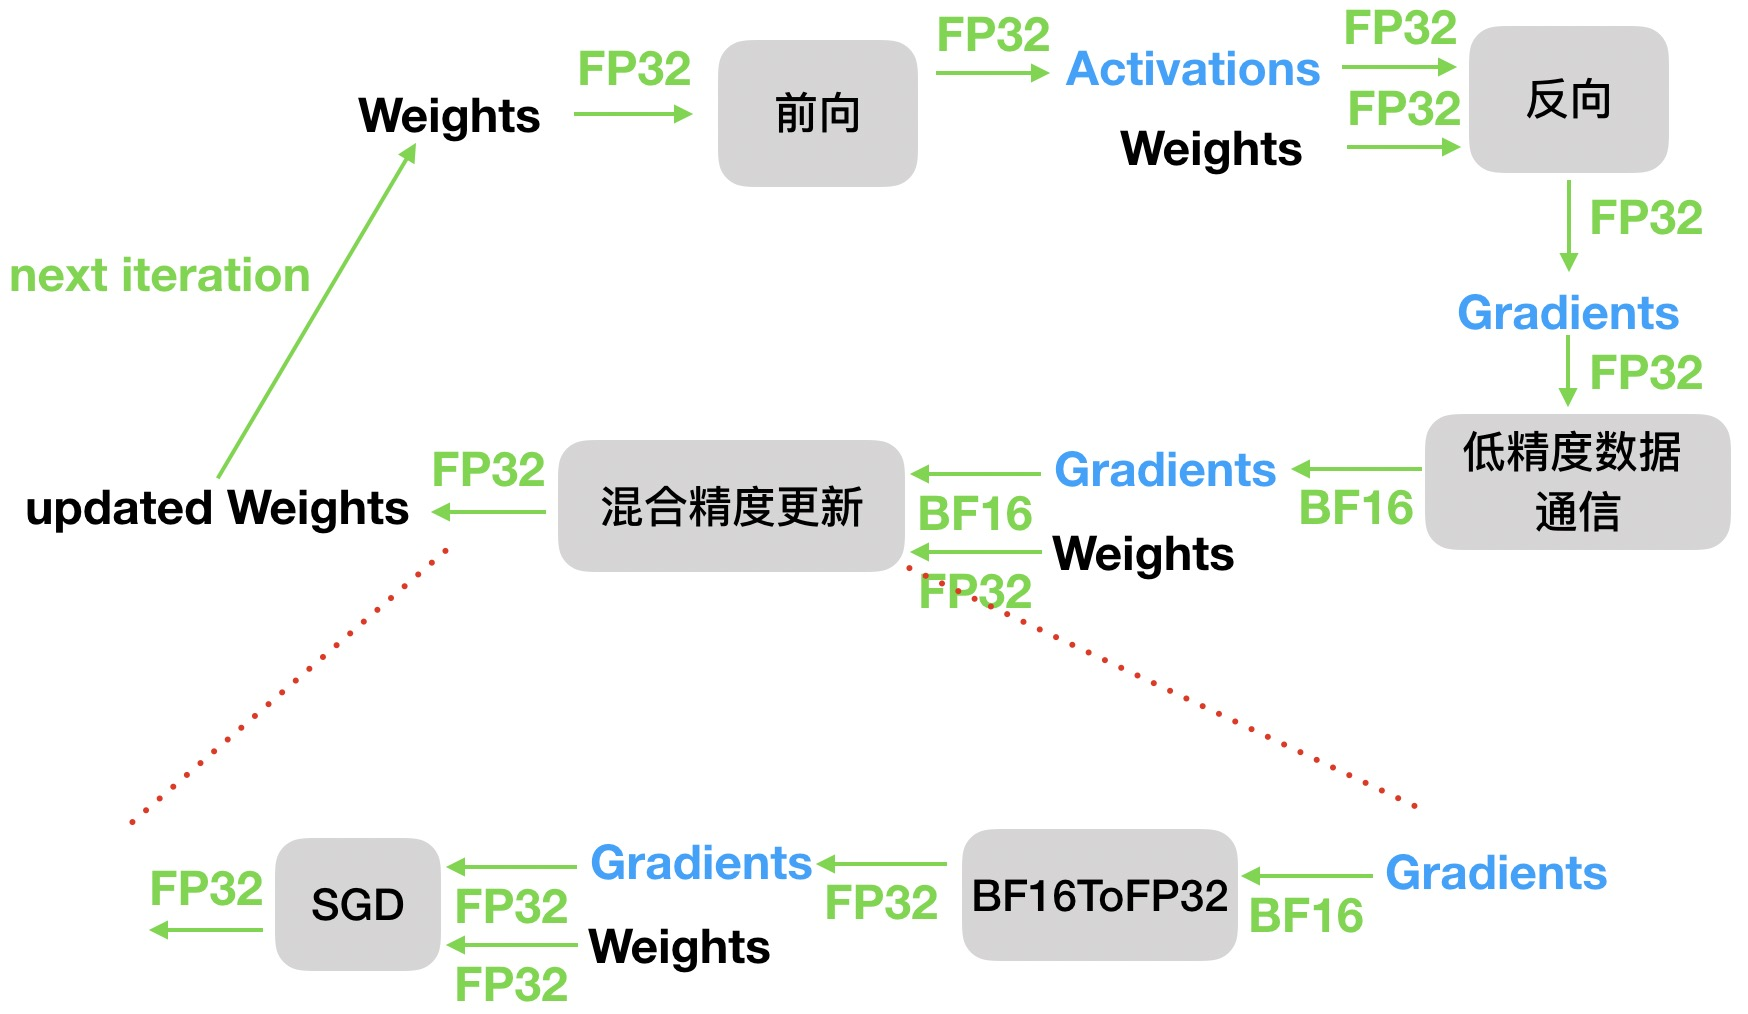
\includegraphics[width=13cm]{MPUflow}
\caption{混合精度更新算法下训练流程图}
\label{fig:MPUflow}
\end{figure}


同理,混合精度更新算法也适用于带动量的SGD,Adagrad,RMSprop等。实验证明混合精度更新算法能够保证在低精度数据通信方式下,神经网络的训练精度达到原始浮点数训练相同精度。

\subsection{LPDU算法设计}
由3.2部分可知,horovod通过继承深度学习框架的优化器实现自定义的分布式优化器DistributedOptimizer达到同步更新的目的。其中DistributedOptimizer的分布式更新算法如算法~\ref{alg:fp32_update}所示。为同步全局梯度,其在调用更新算法之前使用allreduce同步全局梯度,再用全局同步后的梯度更新本地参数,更新后的参数即全局参数。

\begin{algorithm}\small
\caption{原始分布式更新算法}
\textbf{输入:}
本地网络层参数:$Weight$,梯度:$gradient$ \\
\textbf{输出:} 
全局更新后的网络层参数:$Weight$
\begin{algorithmic}[1]
    \STATE{使用$allreduce$对网络层梯度$gradient$做全局同步}
    \STATE{使用更新算法(如随机梯度下降算法),把全局同步后的$gradient$更新到网络层参数$Weight$中}
    \STATE{返回全局更新后的参数$Weight$用于下一次迭代训练}
\end{algorithmic}
	\label{alg:fp32_update}
\end{algorithm}

由3.3.1和3.3.2部分可知,低精度分布式更新算法主要包含两部分:低精度数据通信(LPDC)和混合精度更新(MPU)算法。LPDC算法负责完成BF16格式梯度数据的同步,以减少分布式训练过程中的同步通信量,从而减少同步时间开销,提升分布式训练效率。MPU算法则是为了避免在更新阶段进一步造成精度损失,提出将BF16格式梯度数据转换为浮点数再进行更新的策略。在MPU算法下,使用低精度梯度数据训练神经网络的收敛精度能达到原始浮点数训练相同收敛精度。基于BF16格式数据的LPDU算法如算法~\ref{alg:bf16_update}所示。

\begin{algorithm}\small
\caption{低精度分布式更新算法LPDU}
\textbf{输入:}
本地网络层参数:$Weight$,梯度:$gradient$ \\
\textbf{输出:} 
全局更新后的网络层参数:$Weight$
\begin{algorithmic}[1]
	\STATE{使用LPDC算法求得全局同步后的梯度$gradient_{bf16}$}
    \STATE{使用MPU算法将$gradient_{bf16}$更新到网络层参数$Weight$中}
    \STATE{返回全局更新后的参数$Weight$用于下一次迭代训练}
\end{algorithmic}
	\label{alg:bf16_update}
\end{algorithm}

首先使用LPDC算法完成全局梯度数据的同步,其中通过将原始浮点数据转换为BF16格式数据,在损失部分数据精度情况下减少同步时间开销,以提升分布式训练效率;为避免全局同步后的低精度梯度数据带来的精度损失在更新过程中进一步传播,本文使用MPU算法对模型参数进行更新。LPDU算法下,分布式训练神经网络流程如图~\ref{fig:LPDUflow}所示。实验证明本文提出的低精度分布式更新算法,可在保证神经网络训练精度的前提下,减少分布式训练过程中的同步开销,提升神经网络的训练效率。相关实验结果将在3.4部分详细分析介绍。

\begin{figure}[htp]
\centering
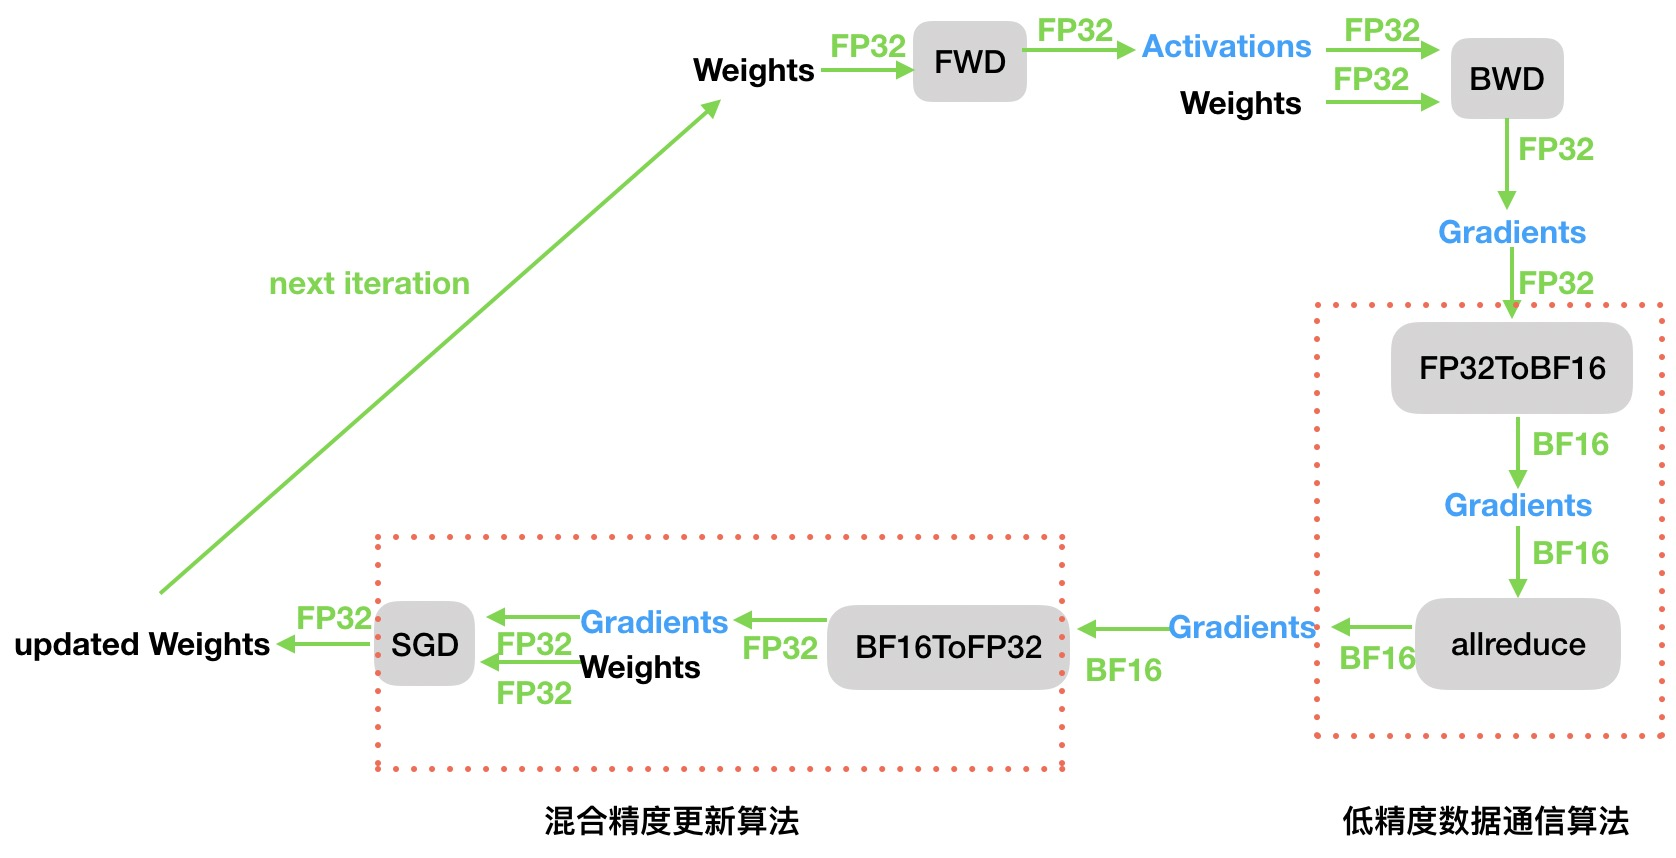
\includegraphics[width=13cm]{LPDUflow}
\caption{低精度分布式更新算法下训练流程图}
\label{fig:LPDUflow}
\end{figure}

\subsection{LPDU算法实现与优化}
由上面内容可知,LPDU算法主要包括两部分:低精度数据通信和混合精度更新算法。其中低精度数据通信算法中主要涉及两个具体实现:1.浮点数到BF16格式数据的转换;2.扩展MPI,使其支持BF16格式数据同步,需要实现一个BF16数据格式的求和函数,供MPI程序在对BF16数据做allreduce时使用。混合精度更新算法中,基于原始SGD算法的实现,只需在其之前实现BF16到FP32数据的转换即可。

综上分析,基于horovod实现LPDU算法,需要完成3部分工作。其中LPDC算法部分工作在3.3.1部分已经介绍。MPU算法部分低精度数据到浮点数到转换部分本文通过在MXNet中的回调函数中实现,实现逻辑如下伪代码所示。在进行低精度数据同步后,程序将自动调用回调函数将低精度梯度转换成浮点数。最后返回给分布式优化器DistributedOptimizer用于模型更新。
\begin{lstlisting}[language=C, numbers=none]
// convert bf16 data to fp32 data on callback function.
void callback() {
        // convert bf16_tensor to fp32, assign to output
        mxnet.tensor.dptr = BF16ToFloat(bf16_pointer, len);
        handle_manager.MarkDone(handle);
        handle_manager.ExecuteCallback(handle);
      }
\end{lstlisting}

为减少LPDU算法中产生的额外数据类型转换开销,以及BF16求和函数的计算效率,我们通过使用intrinsic指令直接操作数据完成数据转换和计算,达到SSE汇编代码相同的性能效果。本文针对不同硬件架构和运行时情况,进行了最优实现。考虑到部分数据地址并不符合AVX512指令地址对齐要求,故需要额外使用movdqu指令处理数据地址不对齐的情况。下面分别是在数据地址满足AVX512指令地址要求和不满足其地址要求情况下,浮点数据转换到BF16数据的具体实现。同理,BF16数据转换到浮点数和BF16 sum中的相关实现与之类似。

\begin{lstlisting}[language=C, numbers=none]
// 数据不对齐情况:使用movdqu指令处理
inline void convert_f32_to_b16(const void* src, void* dst)
{
  __m512i y = _mm512_bsrli_epi128(_mm512_loadu_si512(src), 2);
  _mm256_storeu_si256((__m256i*)(dst), _mm512_cvtepi32_epi16(y));
}

// 数据对齐情况:直接使用intrinsic指令计算
inline void convert_f32_to_b16(__m512i* src, __m256i* dst)
{
  __m512i y = _mm512_bsrli_epi128(*src, 2);
  *dst = _mm512_cvtepi32_epi16(y);
}
\end{lstlisting}

考虑到不同硬件对intrinsic指令对支持程度,本文分别针对LPDU算法中涉及的每种操作进行了三种实现:Naive,AVX256,AVX512以兼容不同硬件。Naive表示不使用任何硬件指令,C代码的实现;AVX256表示使用AVX256相关的硬件指令的实现;同理,AVX512则是使用AVX512硬件指令的实现。如表~\ref{tab:intrinsic_perf}所示。可知相对于Naive实现方法,AVX512实现有2.2~5.7倍的性能提升;AVX256实现有1.6~3.4倍的性能提升。

\begin{longtable}[c]{c*{6}{l}}
\caption{不同实现下性能加速比}\label{tab:intrinsic_perf}\\
\toprule[1.5pt]
 功能函数 & 数组大小 & 
\multicolumn{1}{c}{Naive实现} & \multicolumn{1}{c}{AVX512实现} &
\multicolumn{1}{c}{AVX256实现} & \multicolumn{1}{c}{AVX512} & 
\multicolumn{1}{c}{AVX256} 	\\
\multicolumn{1}{c}{} &\multicolumn{1}{c}{} &\multicolumn{1}{c}{(us)} & \multicolumn{1}{c}{(us)} &
\multicolumn{1}{c}{(us)} & \multicolumn{1}{c}{speedup} &
\multicolumn{1}{c}{speedup} 	\\

\midrule[1pt]%
\endfirsthead%

\multicolumn{7}{c}{续表~\thetable\hskip1em 不同实现下性能加速比}\\

\toprule[1.5pt]
 功能函数 & 数组大小 & 
\multicolumn{1}{c}{原始实现} & \multicolumn{1}{c}{AVX512实现} &
\multicolumn{1}{c}{AVX256实现} & \multicolumn{1}{c}{AVX512} & 
\multicolumn{1}{c}{AVX256} 	\\
\multicolumn{1}{c}{} &\multicolumn{1}{c}{} &\multicolumn{1}{c}{(us)} & \multicolumn{1}{c}{(us)} &
\multicolumn{1}{c}{(us)} & \multicolumn{1}{c}{speedup} &
\multicolumn{1}{c}{speedup} 	\\
\midrule[1pt]%
\endhead%
\hline%

\multicolumn{7}{r}{续下页}%

\endfoot%
\endlastfoot%
F32ToBF16 &	100 & 0.297 & 0.117 & 0.148 & 2.552 & 2.010  \\
F32ToBF16 &	1000 & 2.309 & 0.480 & 0.736 & 4.812 & 3.137  \\
F32ToBF16 &	10000 & 22.612 & 3.923 & 6.183 & 5.763 & 3.657  \\
F32ToBF16 &	100000 & 216.404 & 41.076 & 63.768 & 5.268 & 3.394 \\
F32ToBF16 &	1000000 & 2039.863 & 374.645 & 586.142 & 5.445 & 3.480 \\
BF16ToF32 &	100 & 0.279 & 0.109 & 0.169 & 2.549 & 1.649 \\
BF16ToF32 &	1000 & 2.117 & 0.442 & 0.986 & 4.794 & 2.147 \\
BF16ToF32 &	10000 & 20.492 & 3.795 & 9.129 & 5.400 & 2.245 \\
BF16ToF32 &	100000 & 267.662 & 103.113 & 158.061 & 2.596 & 1.693 \\
BF16ToF32 &	1000000 & 2715.713 & 1188.977 & 1658.944 & 2.284 & 1.637 \\
BF16 sum &	100 & 0.456 & 0.200 & 0.314 & 2.285 & 1.453 \\
BF16 sum &	1000 & 3.993 & 1.089 & 2.528 & 3.665 & 1.579 \\
BF16 sum &	10000 & 39.258 & 9.740 & 23.867 & 4.031 & 1.645 \\
BF16 sum &	100000 & 404.553 & 113.089 & 253.198 & 3.577 & 1.598 \\
BF16 sum &	1000000 & 3898.513 & 981.624 & 2390.526 & 3.971 & 1.631 \\
\bottomrule[1.5pt]
\end{longtable}

\section{实验与分析}
为说明低精度分布式更新算法的有效性,本节将从神经网络的训练性能和精度两方面进行对比分析。同时,为了说明LPDU算法的普适性,我们将分别展示图像分类、物体检测等领域网络在LPDU算法下的训练结果。为验证LPDU算法的高效性,本节将单独比较原始分布式更新算法与低精度分布式更新算法的效率。同时对实验细节和数据集也进行了详细介绍,使得实验结果和分析更具说服力。

\subsection{数据集介绍}
为说明本章提出的低精度分布式更新算法的广泛适用性。本章分别从典型的图像分类、物体检测应用中选择有代表性的神经网络在各自领域公开数据集上进行实验,分别与原始训练结果进行对比,验证低精度分布式更新算法的有效性。数据集信息如表~\ref{tab:datasets}所示。

ILSVRC2012: ImageNet数据集,包含1281167张图片,1000个类别,总容量约140GB,是图像分类领域公认的权威数据集。

PASCAL VOC: 为图像识别和分类提供了一整套标准化数据。本文使用其2007与2012年发布的数据集,用于训练物体检测网。包含16551个有效物体框,共20个类别,总容量约2.8GB。

\begin{table}[htbp]
\centering
\begin{minipage}[t]{0.9\linewidth}
\caption{数据集概况}
\label{tab:datasets}
\begin{tabularx}{\linewidth}{l X X X }
\toprule[1.5pt]
{\song 数据集名称} & {\song 适用场景} & {\song 样本数量} & {	\song 类别数量}\\
\midrule[1pt]
ILSVRC2012 & 图像分类 & 1281167 & 1000\\
VOC2007+2012 & 目标检测 & 16551 & 20\\
\bottomrule[1.5pt]
\end{tabularx}
\end{minipage}
\end{table}

\subsection{实验环境介绍}
本文使用的软件主要有:MXNet 1.3版本,OpenMPI 4.0以及开源框架horovod。本章LPDU算法则是在ctcyang/horovod:mxnet feature fp16分支基础上进一步设计实现的。所有实验均是在双sockets的Xeon Gold 6148处理器的集群中运行所得的结果。因为目前各个框架CPU端计算性能均基于单socket进行优化。在每个socket上跑一个训练实例可使训练效率达到最佳。故本文在每个机器节点上跑两个训练实例,使得每个socket上跑一个训练实例,以充分发挥CPU计算性能。

\subsection{LPDU算法性能分析}
由3.3部分算法分析可知,LPDU算法开销包含四部分时间开销:通信时间、FP32数据转换BF16数据开销、对BF16数据求和开销、BF16数据转换为FP32数据开销;原始更新算法开销包含两部分时间开销:通信开销与FP32数据求和开销。在不同数据规模下,测得8节点16实例实验环境中原始更新算法与LPDU算法时间开销如下表~\ref{tab:fp32_bf16_update_time}所示。可知在数据量大于10,000时,LPDU算法相对于原始更新算法有加速。随着数据量的增大,加速效果越明显;当数据量增大到1,000,000时,LPDU算法加速比能达到1.35,可以预测数据量越大,通信开销占比越大,BF16更新算法加速比也将进一步增大。

\begin{table}[htbp]
  \centering
  \caption{不同数据规模下两种更新算法时间开销}
  \label{tab:fp32_bf16_update_time}
  \begin{minipage}[t]{0.8\textwidth} 
    \begin{tabularx}{\linewidth}{|l|X|X|X|}
      \hline
      数组大小  & origin alg$^{*}$(us) & LPDU alg$^{**}$(us) & Speedup\\
      \hline
100 & 6842.00 & 6332.42 & 1.08 \\
1000 & 5213.00 & 5216.59 & 1.00 \\
10000 & 6317.00 & 6204.70 & 1.02 \\
100000 & 7245.00 & 6081.76 & 1.19 \\
1000000 & 20668.00 & 15259.92 & 1.35 \\
      \hline
    \end{tabularx}\\[2pt]
    \footnotesize
    *:原始分布式更新算法时间开销:通信和浮点数求和时间\\
    **:低精度分布式更新算法时间开销:FP32ToBF16,BF16ToFP32,通信和BF16求和时间
  \end{minipage}
\end{table}

本节以50层的Resnet网络为例,从理论上分析该网络在8节点16训练实例环境中,LPDU算法相对于原始更新算法的理论性能收益。 由表~\ref{tab:resnet50_params}可知,仅有2.8\%的参数的数据规模小于100,000;97.2\%参数的规模均大于100,000;64.57\%参数的规模大于1,000,000。根据表~\ref{tab:fp32_bf16_update_time}数据可知:在50层的Resnet网络中,LPDU算法相对于原始更新算法的更新时间将有1.19~1.35倍的加速,甚至大于1.35倍的加速。

\begin{table}[htbp]
\centering
\begin{minipage}[t]{0.9\linewidth}
\caption{Resnet50各层参数大小分布}
\label{tab:resnet50_params}
\begin{tabularx}{\linewidth}{l X X }
\toprule[1.5pt]
{\song 参数规模} & {\song 参数个数} & {\song 占比(\%)}\\
\midrule[1pt]
<100000 & 713920 & 2.80 \\
100000-1000000 & 8323072 & 32.63 \\
>1000000 & 16466920 & 64.57 \\
\bottomrule[1.5pt]
\end{tabularx}
\end{minipage}
\end{table}

在50层Resnet网络的真实训练场景中,原始更新算法与LPDU算法在不同训练实例个数的更新时间如表~\ref{tab:fp32_bf16_real_update_time}所示。在8节点16实例情况下,LPDU算法相对于原始更新算法的更新时间有1.3倍的性能提升,在8节点情况下同步时间由原始的0.458s降低至0.352s,可节省30\%的更新时间。与表~\ref{tab:fp32_bf16_update_time}和上述分析1.19~1.35倍的性能提升相一致。两者相互验证,说明了算法实现的正确性和有效性。 

\begin{table}[htbp]
  \centering
  \caption{不同训练实例中两种算法更新时间}
  \label{tab:fp32_bf16_real_update_time}
  \begin{minipage}[t]{0.8\textwidth} 
    \begin{tabularx}{\linewidth}{|l|X|X|X|X|}
      \hline
      节点数 & 实例数 & origin alg(s) & LPDU alg(s) & Speedup\\
      \hline
1 & 1 & 0.015 & 0.041 & 0.366 \\
1 & 2 & 0.075 & 0.076 & 0.987 \\
2 & 4 & 0.374 & 0.299 & 1.251 \\
4 & 8 & 0.428 & 0.337 & 1.270 \\
8 & 16 & 0.458 & 0.352 & 1.301 \\
      \hline
    \end{tabularx}\\[2pt]
    \footnotesize
    说明:每个实例配置均为resnet50, batch size=128\\
  \end{minipage}
\end{table}

为进一步比较原始更新算法与LPDU算法在实际训练过程中的性能差异,本节通过采样得到不同训练实例下,实际训练中每次迭代时间如表~\ref{tab:fp32_bf16_real_iter_time}所示。可知在8节点16训练实例情况下,LPDU算法的单次迭代时间相对于原始更新算法减少了0.12s,其来自于BF16算法同步时间的降低。该时间与表~\ref{tab:fp32_bf16_real_update_time}中同步时间减少部分相一致。因为LPDU算法降低了同步时间开销,使得分布式训练效率相对于原始更新算法有所提升。如在8节点16训练实例情况下,LPDU算法使得分布式训练效率由84.05\%提升至87.5\%,提升了3.5个百分点。不可否认,现阶段CPU训练神经网络速度远慢于GPU训练,使得分布式训练中通信压力相对较小。若使用GPU训练,单次迭代中计算时间将大大减少,使得同步时间占比增大。此时LPDU算法对提升分布式训练效率的作用将更加明显。

\begin{table}[htbp]
  \centering
  \caption{不同训练实例中两种算法迭代时间}
  \label{tab:fp32_bf16_real_iter_time}
  \begin{minipage}[t]{0.9\textwidth} 
    \begin{tabularx}{\linewidth}{|l|X|X|X|X|X|}
      \hline
      节点数 & 实例数 & origin time & LPDU time & origin & LPDU \\
       &  & (s/iter) & (s/iter) & scaling & scaling\\
      \hline
1 & 1 & 2.8158 & 2.8271 & 100.00 & 100.00 \\
1 & 2 & 2.8685 & 2.9990 & 98.16 & 94.27 \\
2 & 4 & 3.0450 & 3.0387 & 92.47 & 93.04 \\
4 & 8 & 3.3332 & 3.1877 & 84.48 & 88.69 \\
8 & 16 & 3.3501 & 3.2310 & 84.05 & 87.50 \\
      \hline
    \end{tabularx}\\[2pt]
    \footnotesize
    说明:每个实例配置均为resnet50, batch size=128\\
  \end{minipage}
\end{table}

由上述分析可知,神经网络的参数量越大,受网络带宽限制,同步开销越大,LPDU算法对分布式性能提升作用越大。同时,该算法普遍适用于各种主流神经网络,如图像分类,物体检测和递归循环网络等。表~\ref{tab:ssd_vgg_scaling}分别展示了LPDU算法在物体检测网络SSD和分类网VGG中的性能提升。可知模型稍小的SSD网络中,LPDU算法可使分布式训练效率由85.01\%提升至89.84\%,相对于原始更新算法提升了4.83个百分点;在模型较大的VGG网络中该算法性能提升更加明显,相对于原始更新算法,在8节点16训练实例情况下提升了7.13\%。
\begin{table}[htbp]
  \centering
  \caption{原始更新算法与BF16更新算法在SSD与VGG网络中的性能加速}
  \label{tab:ssd_vgg_scaling}
  \begin{minipage}[t]{0.8\textwidth} 
    \begin{tabularx}{\linewidth}{|l|X|X|X|X|}
      \hline
      实例数 & SSD$^{*}$ FP32 & SSD BF16 & VGG$^{**}$ FP32 & VGG BF16 \\
       & scaling & scaling & scaling & scaling\\
      \hline
1 & 100.00 & 100.00 & 100.00 & 100.00 \\
2 & 96.88 & 97.81 & 88.78 & 92.17 \\
4 & 91.97 & 95.18 & 86.65 & 90.06 \\
8 & 88.44 & 92.27 & 83.48 & 89.44 \\
16 & 85.01 & 89.84 & 79.42 & 86.55 \\
      \hline
    \end{tabularx}\\[2pt]
    \footnotesize
    *:SSD的模型大小为101MB\\
    **:VGG的模型大小为528MB
  \end{minipage}
\end{table}

\subsection{LPDU算法精度比较}
为说明LPDU算法不会对神经网络精度造成影响,本节分别比较在相同配置下,原始更新算法和LPDU算法下神经网络最终的收敛精度。图~\ref{fig:resnet50_4node_acc}为4节点8实例情况下原始更新算法与LPDU算法下Resnet50的收敛曲线。可知在训练集与验证集上LPDU算法均与原始更新算法的精度曲线基本重合,最终精度也保持一致,说明LPDU算法在分类网中不会造成网络的精度损失。不同节点实例下原始更新算法与LPDU算法在ImageNet数据集上的最终结果如表~\ref{tab:resnet50_diff_node_acc}所示。可知相同节点数下,LPDU算法与原始更新算法下收敛精度差距不超过0.3\%,该细微误差属于网络训练过程中的正常波动。说明不同节点下LPDU算法均能保证神经网络的训练精度收敛到理想精度,验证了LPDU算法的有效性与正确性。

\begin{figure}[htp]
\centering
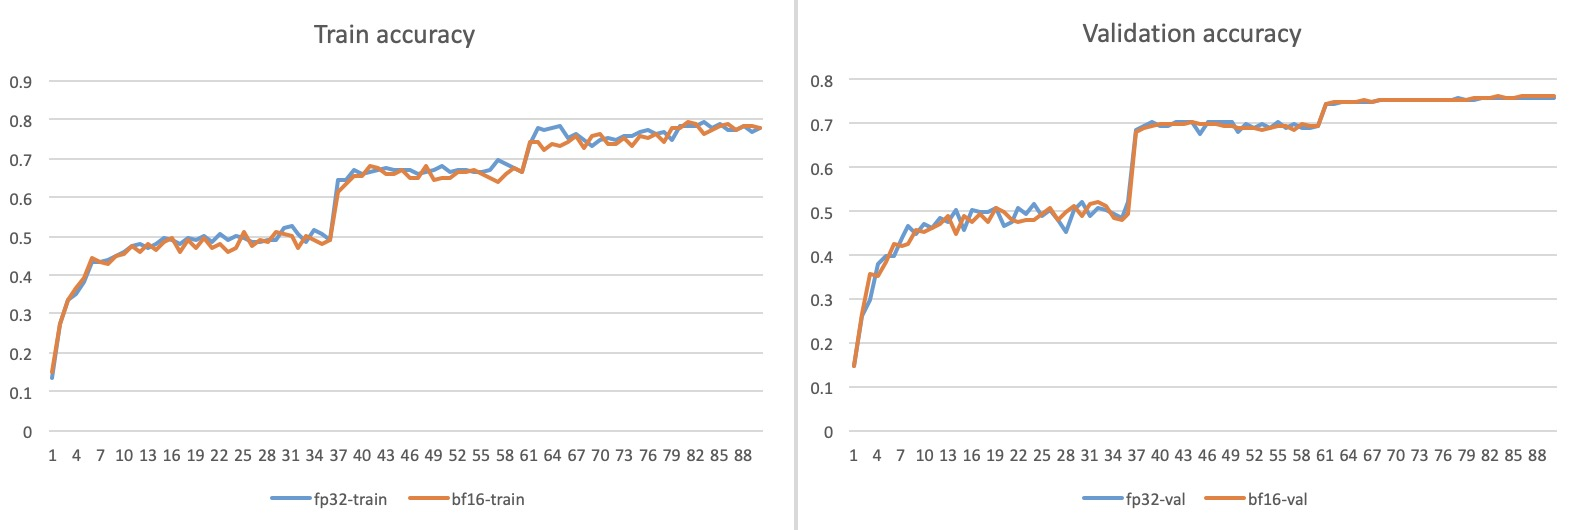
\includegraphics[width=13cm]{resnet50_4node_acc}
\caption{Resnet50中原始更新算法与LPDU算法收敛曲线}
\label{fig:resnet50_4node_acc}
\end{figure}

\begin{table}[htbp]
\centering
\begin{minipage}[t]{0.9\linewidth}
\caption{Resnet50在不同节点数下最终精度}
\label{tab:resnet50_diff_node_acc}
\begin{tabularx}{\linewidth}{l X X X }
\toprule[1.5pt]
{\song 数据集} & {\song 节点数} & {\song 原始更新算法(\%)} & {	\song LPDU算法(\%)}\\
\midrule[1pt]
ILSVRC2012 & 1 &  76.18 & 76.15\\
ILSVRC2012 & 4 & 76.20 & 75.98\\
ILSVRC2012 & 8 & 76.08 & 76.13\\
\bottomrule[1.5pt]
\end{tabularx}
\end{minipage}
\end{table}
为验证LPDU算法对神经网络的普遍适用性,本节以物体检测领域经典网络SSD为例,使用LPDU算法对其进行训练,通过比较原始更新算法与本文算法在验证集的收敛曲线和最终收敛结果验证LPDU算法的有效性。如图~\ref{fig:ssd_4node_acc}所示:在4节点8实例情况下,LPDU算法与原始更新算法在验证集上的mAP曲线基本重合,说明LPDU算法在物体检测网络中不会造成网络的精度损失。不同节点实例下原始更新算法与LPDU算法在VOC数据集上的最终结果如表~\ref{tab:ssd_diff_node_acc}所示,可知相同节点数下,LPDU算法与原始更新算法下验证集结果差距不超过0.4\%,在正常数据波动范围内。该误差来源于神经网络正常训练误差和BF16数据造成的部分数据损失。说明不同节点情况下LPDU算法均能保证神经网络的训练精度收敛到原始FP32更新算法相接近的精度,验证了LPDU算法的有效性与正确性。 

\begin{figure}[htp]
\centering
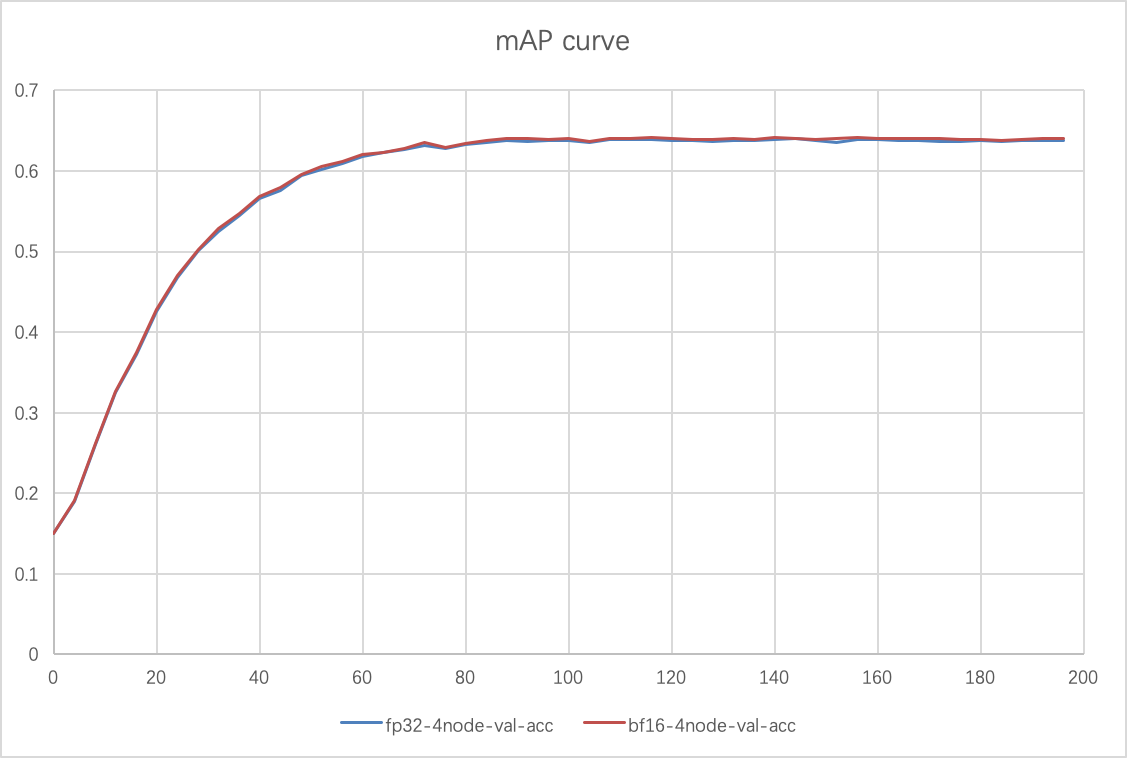
\includegraphics[width=10cm]{ssd_4node_acc}
\caption{SSD中原始更新算法与LPDU算法收敛曲线}
\label{fig:ssd_4node_acc}
\end{figure}


\begin{table}[htbp]
\centering
\begin{minipage}[t]{0.9\linewidth}
\caption{ssd在不同节点数下最终精度}
\label{tab:ssd_diff_node_acc}
\begin{tabularx}{\linewidth}{l X X X }
\toprule[1.5pt]
{\song 数据集} & {\song 节点数} & {\song 原始更新算法(\%)} & {	\song LPDU算法(\%)}\\
\midrule[1pt]
VOC2007+2012 & 1 & 64.22 & 64.18\\
VOC2007+2012 & 4 & 64.00 & 64.06\\
VOC2007+2012 & 8 & 64.04 & 63.64\\
\bottomrule[1.5pt]
\end{tabularx}
\end{minipage}
\end{table}

\section{本章小结}
本章主要提出了低精度分布式更新算法以减小分布式训练过程中同步时间的开销,提升分布式训练神经网络的效率,同时保证神经网络训练精度达到原始浮点数训练相同精度。首先介绍了将horovod整合进MXNet的设计原理,然后介绍了LPDU算法中的两个算法组成:低精度数据通信LPDC和混合精度更新MPU算法。并分别介绍了LPDC算法和MPU算法的原理和设计思想;并进一步在此基础上介绍了LPDU算法的设计和实现,以及LPDU算法实现过程中优化性能的相关方法。最后对LPDU算法中各个模块的时间开销进行了详细分析,验证本章算法的高效性。最后将该算法用于训练分类网和物体检测网,通过比较LPDU算法与原始更新算法的训练效率与神经网络最终的收敛精度,说明了本章算法在不影响神经网络训练精度情况下,使得分布式训练效率有明显提升。也说明了LPDU算法对神经网络的普遍适用性。
